\documentclass{article}
\usepackage{tikz}

\usepackage{circuitikz}
\usetikzlibrary{circuits}
\usetikzlibrary{circuits.plc.ladder}


\begin{document}
	\begin{center}
		
		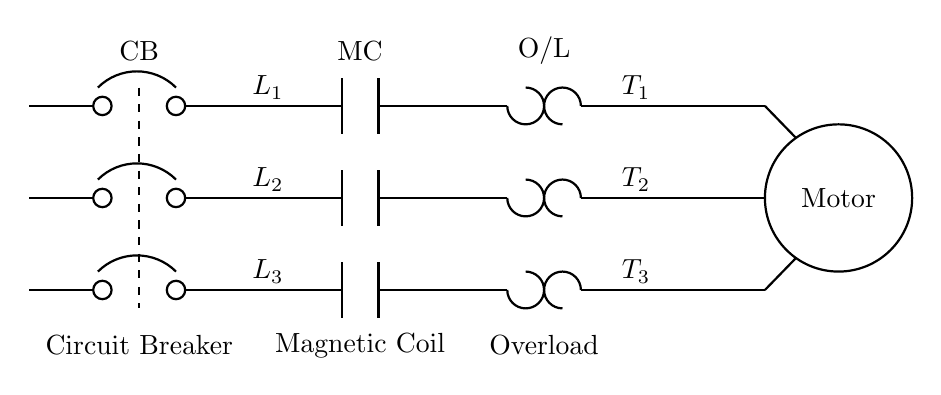
\begin{tikzpicture}[circuit plc ladder,thick,ladderrungsep=0.8,scale=0.19]
			
			% Draw a coordinate system
			%\draw[->] (-40,0) -- (40,0) node[right] {$x$};
			%\draw[->] (0,-40) -- (0,40) node[above] {$y$};	
			%\draw (-9,0) to [contact NO] (-6,0) ;
			
			%draw N.O. relay		
			%draw N.O. relay	
			%draw N.O. relay	
			
			% Set the coordinates for the line
			\coordinate (start) at (-9,1.5);
			\coordinate (end) at (-9,-1.5);
			% Draw the red V-line
			\draw (start) -- (end);
			% Set the coordinates for the line
			\coordinate (start) at (-11,1.5);
			\coordinate (end) at (-11,-1.5);
			% Draw the red V-line
			\draw (start) -- (end);		
			
			% Set the coordinates for the line
			\coordinate (start) at (-9,0);
			\coordinate (end) at (-4,0);
			% Draw the red V-line
			\draw (start) -- (end);
			% Set the coordinates for the line
			\coordinate (start) at (-11,0);
			\coordinate (end) at (-16,0);
			% Draw the red V-line
			\draw  (start) -- (end);
			
			
			
			% Set the coordinates for the line
			\coordinate (start) at (-9,6.5);
			\coordinate (end) at (-9,3.5);
			% Draw the red V-line
			\draw (start) -- (end);
			% Set the coordinates for the line
			\coordinate (start) at (-11,6.5);
			\coordinate (end) at (-11,3.5);
			% Draw the red V-line
			\draw (start) -- (end);
			
			% Set the coordinates for the line
			\coordinate (start) at (-9,5);
			\coordinate (end) at (-4,5);
			% Draw the red V-line
			\draw (start) -- (end);
			% Set the coordinates for the line
			\coordinate (start) at (-11,5);
			\coordinate (end) at (-16,5);
			% Draw the red V-line
			\draw (start) -- (end);
			
			% Set the coordinates for the line
			\coordinate (start) at (-9,-6.5);
			\coordinate (end) at (-9,-3.5);
			% Draw the red V-line
			\draw (start) -- (end);
			% Set the coordinates for the line
			\coordinate (start) at (-11,-6.5);
			\coordinate (end) at (-11,-3.5);
			% Draw the red V-line
			\draw (start) -- (end);
			
			% Set the coordinates for the line
			\coordinate (start) at (-9,-5);
			\coordinate (end) at (-4,-5);
			% Draw the red V-line
			\draw (start) -- (end);
			% Set the coordinates for the line
			\coordinate (start) at (-11,-5);
			\coordinate (end) at (-16,-5);
			% Draw the red V-line
			\draw (start) -- (end);	
			
			% draw OL
			% draw OL		
			% draw OL
			
			% Set the center and radius of the arc
			\coordinate (center) at (-2,1);
			\def\radius{1}
			
			% Draw the arc
			\draw (center) ++(0:\radius) arc (90:-180:\radius);
			
			% Optional: Mark the center
			%	\filldraw (center) circle (2pt) node[below right, black] {$(x_0, y_0)$};
			
			% Set the coordinates for the line
			\coordinate (start) at (-4,0);
			\coordinate (end) at (-2,0);
			
			% Draw the red line
			\draw (start) -- (end);
			
			%draw second OL on top
			
			% Set the center and radius of the arc
			\coordinate (center) at (-2,6);
			\def\radius{1}
			
			% Draw the arc
			\draw (center) ++(0:\radius) arc (90:-180:\radius);
			
			% Optional: Mark the center
			%	\filldraw (center) circle (2pt) node[below right, black] {$(x_0, y_0)$};
			
			% Set the coordinates for the line
			\coordinate (start) at (-4,5);
			\coordinate (end) at (-2,5);
			
			% Draw the red line
			\draw (start) -- (end);	
			
			%draw third OL on bottom
			
			% Set the center and radius of the arc
			\coordinate (center) at (-2,-4);
			\def\radius{1}
			
			% Draw the arc
			\draw (center) ++(0:\radius) arc (90:-180:\radius);
			
			% Optional: Mark the center
			%	\filldraw (center) circle (2pt) node[below right, black] {$(x_0, y_0)$};
			
			% Set the coordinates for the line
			\coordinate (start) at (-4,-5);
			\coordinate (end) at (-2,-5);
			
			% Draw the red line
			\draw (start) -- (end);	
			
			
			% Draw right OL		
			\coordinate (center) at (0,-1);
			\def\radius{1}
			
			% Draw the arc
			\draw (center) ++(0:\radius) arc (270:0:\radius);
			% Optional: Mark the center
			%	\filldraw (center) circle (2pt) node[below right, black] {$(x_1, y_1)$};		
			% Set the coordinates for the line
			\coordinate (start) at (2,0);
			\coordinate (end) at (6,0);
			
			% Draw the red line
			\draw (start) -- (end);	
			
			% Draw top the arc
			
			\coordinate (center) at (0,4);
			\def\radius{1}		
			
			\draw (center) ++(0:\radius) arc (270:0:\radius);
			% Optional: Mark the center
			%\filldraw (center) circle (2pt) node[below right, black] {$(x_1, y_1)$};		
			% Set the coordinates for the line
			\coordinate (start) at (2,5);
			\coordinate (end) at (6,5);
			
			% Draw the red line
			\draw (start) -- (end);			
			
			% Draw bottom the arc
			
			\coordinate (center) at (0,-6);
			\def\radius{1}		
			
			\draw (center) ++(0:\radius) arc (270:0:\radius);
			% Optional: Mark the center
			%\filldraw (center) circle (2pt) node[below right, black] {$(x_1, y_1)$};		
			% Set the coordinates for the line
			\coordinate (start) at (2,-5);
			\coordinate (end) at (6,-5);
			
			% Draw the red line
			\draw (start) -- (end);	
			
			%draw three phase motor
			%draw three phase motor
			%draw three phase motor
			
			
			% Set the coordinates for the line
			\coordinate (start) at (6,-5);
			\coordinate (end) at (12,-5);
			
			% Draw the blue line
			
			\draw(start) -- (end);	
			
			\draw(end) -- (13.7,-3.25);
			
			% Set the coordinates for the line
			\coordinate (start) at (6,0);
			\coordinate (end) at (12,0);
			
			% Draw the red line
			\draw(start) -- (end);
			
			% Set the coordinates for the line
			\coordinate (start) at (6,5);
			\coordinate (end) at (12,5);
			
			% Draw the red line
			\draw(start) -- (end);
			
			\draw(end) -- (13.7,3.25);
			
			%draw a circle
			%draw a circle
			%draw a circle
			
			\draw(16,0) circle [radius=4] node at (16,0) {Motor};
			% add OL and MC
			
			\node at (0,8) {O/L};
			\node at (0,-8) {Overload};
			
			\node at (-10,8) {MC}; 
			\node at (-10,-8) {Magnetic Coil}; 	 
			
			% add L1/L2/L3		
			\node at (-15,6) {$L_1$};  
			\node at (-15,1) {$L_2$}; 
			\node at (-15,-4) {$L_3$};  
			
			% add T1/T2/T3		
			\node at (5,6) {$T_1$};  
			\node at (5,1) {$T_2$}; 
			\node at (5,-4) {$T_3$};  
			
			
			
			% draw circuit breaker 
			
			\draw(-20,0) circle [radius=0.5] ;
			\draw(-24,0) circle [radius=0.5] ; 
			% Set the center and radius of the arc
			\coordinate (center) at (-23,1);
			\def\radius{3}
			
			% Draw the arc
			\draw (center) ++(0:\radius) arc (45:135:\radius); 
			%-----------------------------------------------
			\draw(-20,5) circle [radius=0.5] ;
			\draw(-24,5) circle [radius=0.5] ; 
			% Set the center and radius of the arc
			\coordinate (center) at (-23,6);
			\def\radius{3}
			
			% Draw the arc
			\draw (center) ++(0:\radius) arc (45:135:\radius);  
			%-----------------------------------------------
			\draw(-20,-5) circle [radius=0.5] ;
			\draw(-24,-5) circle [radius=0.5] ; 
			% Set the center and radius of the arc
			\coordinate (center) at (-23,-4);
			\def\radius{3}
			
			% Draw the arc
			\draw (center) ++(0:\radius) arc (45:135:\radius); 
			%-----------------------------------------------
			
			
			% Set the coordinates for the line
			\coordinate (start) at (-19.5,0);
			\coordinate (end) at (-16,0);
			% Draw the red V-line
			\draw (start) -- (end);
			
			% Set the coordinates for the line
			\coordinate (start) at (-24.5,0);
			\coordinate (end) at (-28,0);
			% Draw the red V-line
			\draw (start) -- (end);
			%-----------------------------------------------
			
			% Set the coordinates for the line
			\coordinate (start) at (-19.5,5);
			\coordinate (end) at (-16,5);
			% Draw the red V-line
			\draw (start) -- (end);
			
			% Set the coordinates for the line
			\coordinate (start) at (-24.5,5);
			\coordinate (end) at (-28,5);
			% Draw the red V-line
			\draw (start) -- (end);
			%-----------------------------------------------
			
			% Set the coordinates for the line
			\coordinate (start) at (-19.5,-5);
			\coordinate (end) at (-16,-5);
			% Draw the red V-line
			\draw (start) -- (end);
			
			% Set the coordinates for the line
			\coordinate (start) at (-24.5,-5);
			\coordinate (end) at (-28,-5);
			% Draw the red V-line
			\draw (start) -- (end);
			%-----------------------------------------------  
			% Set the coordinates for the line
			\coordinate (start) at (-22,6);
			\coordinate (end) at (-22,-6);		
			\draw[dashed, black] (start) -- (end) node at (-22,-8) {Circuit Breaker};		
			%\node at (-10,-8) {Magnetic Coil}; 	
			\node at (-22,8) {CB}; 
			%\node at (-10,-8) {Magnetic Coil}; 			
		\end{tikzpicture}
	\end{center}	
	
 
	\begin{figure} [ht]
		
		\caption{Typical AC Motor Control Diagram}
		
	\end{figure}
\end{document}